\PassOptionsToPackage{unicode=true}{hyperref} % options for packages loaded elsewhere
\PassOptionsToPackage{hyphens}{url}
%
\documentclass[ignorenonframetext,]{beamer}
\usepackage{pgfpages}
\setbeamertemplate{caption}[numbered]
\setbeamertemplate{caption label separator}{: }
\setbeamercolor{caption name}{fg=normal text.fg}
\beamertemplatenavigationsymbolsempty
\usepackage{lmodern}
\usepackage{amssymb,amsmath}
\usepackage{ifxetex,ifluatex}
\usepackage{fixltx2e} % provides \textsubscript
\ifnum 0\ifxetex 1\fi\ifluatex 1\fi=0 % if pdftex
  \usepackage[T1]{fontenc}
  \usepackage[utf8]{inputenc}
  \usepackage{textcomp} % provides euro and other symbols
\else % if luatex or xelatex
  \usepackage{unicode-math}
  \defaultfontfeatures{Ligatures=TeX,Scale=MatchLowercase}
\fi
\usetheme[]{CambridgeUS}
\usecolortheme{beaver}
\usefonttheme{structurebold}
% use upquote if available, for straight quotes in verbatim environments
\IfFileExists{upquote.sty}{\usepackage{upquote}}{}
% use microtype if available
\IfFileExists{microtype.sty}{%
\usepackage[]{microtype}
\UseMicrotypeSet[protrusion]{basicmath} % disable protrusion for tt fonts
}{}
\IfFileExists{parskip.sty}{%
\usepackage{parskip}
}{% else
\setlength{\parindent}{0pt}
\setlength{\parskip}{6pt plus 2pt minus 1pt}
}
\usepackage{hyperref}
\hypersetup{
            pdftitle={B5 Simple Features},
            pdfauthor={Jan-Philipp Kolb},
            pdfborder={0 0 0},
            breaklinks=true}
\urlstyle{same}  % don't use monospace font for urls
\newif\ifbibliography
\usepackage{color}
\usepackage{fancyvrb}
\newcommand{\VerbBar}{|}
\newcommand{\VERB}{\Verb[commandchars=\\\{\}]}
\DefineVerbatimEnvironment{Highlighting}{Verbatim}{commandchars=\\\{\}}
% Add ',fontsize=\small' for more characters per line
\usepackage{framed}
\definecolor{shadecolor}{RGB}{248,248,248}
\newenvironment{Shaded}{\begin{snugshade}}{\end{snugshade}}
\newcommand{\AlertTok}[1]{\textcolor[rgb]{0.94,0.16,0.16}{#1}}
\newcommand{\AnnotationTok}[1]{\textcolor[rgb]{0.56,0.35,0.01}{\textbf{\textit{#1}}}}
\newcommand{\AttributeTok}[1]{\textcolor[rgb]{0.77,0.63,0.00}{#1}}
\newcommand{\BaseNTok}[1]{\textcolor[rgb]{0.00,0.00,0.81}{#1}}
\newcommand{\BuiltInTok}[1]{#1}
\newcommand{\CharTok}[1]{\textcolor[rgb]{0.31,0.60,0.02}{#1}}
\newcommand{\CommentTok}[1]{\textcolor[rgb]{0.56,0.35,0.01}{\textit{#1}}}
\newcommand{\CommentVarTok}[1]{\textcolor[rgb]{0.56,0.35,0.01}{\textbf{\textit{#1}}}}
\newcommand{\ConstantTok}[1]{\textcolor[rgb]{0.00,0.00,0.00}{#1}}
\newcommand{\ControlFlowTok}[1]{\textcolor[rgb]{0.13,0.29,0.53}{\textbf{#1}}}
\newcommand{\DataTypeTok}[1]{\textcolor[rgb]{0.13,0.29,0.53}{#1}}
\newcommand{\DecValTok}[1]{\textcolor[rgb]{0.00,0.00,0.81}{#1}}
\newcommand{\DocumentationTok}[1]{\textcolor[rgb]{0.56,0.35,0.01}{\textbf{\textit{#1}}}}
\newcommand{\ErrorTok}[1]{\textcolor[rgb]{0.64,0.00,0.00}{\textbf{#1}}}
\newcommand{\ExtensionTok}[1]{#1}
\newcommand{\FloatTok}[1]{\textcolor[rgb]{0.00,0.00,0.81}{#1}}
\newcommand{\FunctionTok}[1]{\textcolor[rgb]{0.00,0.00,0.00}{#1}}
\newcommand{\ImportTok}[1]{#1}
\newcommand{\InformationTok}[1]{\textcolor[rgb]{0.56,0.35,0.01}{\textbf{\textit{#1}}}}
\newcommand{\KeywordTok}[1]{\textcolor[rgb]{0.13,0.29,0.53}{\textbf{#1}}}
\newcommand{\NormalTok}[1]{#1}
\newcommand{\OperatorTok}[1]{\textcolor[rgb]{0.81,0.36,0.00}{\textbf{#1}}}
\newcommand{\OtherTok}[1]{\textcolor[rgb]{0.56,0.35,0.01}{#1}}
\newcommand{\PreprocessorTok}[1]{\textcolor[rgb]{0.56,0.35,0.01}{\textit{#1}}}
\newcommand{\RegionMarkerTok}[1]{#1}
\newcommand{\SpecialCharTok}[1]{\textcolor[rgb]{0.00,0.00,0.00}{#1}}
\newcommand{\SpecialStringTok}[1]{\textcolor[rgb]{0.31,0.60,0.02}{#1}}
\newcommand{\StringTok}[1]{\textcolor[rgb]{0.31,0.60,0.02}{#1}}
\newcommand{\VariableTok}[1]{\textcolor[rgb]{0.00,0.00,0.00}{#1}}
\newcommand{\VerbatimStringTok}[1]{\textcolor[rgb]{0.31,0.60,0.02}{#1}}
\newcommand{\WarningTok}[1]{\textcolor[rgb]{0.56,0.35,0.01}{\textbf{\textit{#1}}}}
\usepackage{graphicx,grffile}
\makeatletter
\def\maxwidth{\ifdim\Gin@nat@width>\linewidth\linewidth\else\Gin@nat@width\fi}
\def\maxheight{\ifdim\Gin@nat@height>\textheight\textheight\else\Gin@nat@height\fi}
\makeatother
% Scale images if necessary, so that they will not overflow the page
% margins by default, and it is still possible to overwrite the defaults
% using explicit options in \includegraphics[width, height, ...]{}
\setkeys{Gin}{width=\maxwidth,height=\maxheight,keepaspectratio}
% Prevent slide breaks in the middle of a paragraph:
\widowpenalties 1 10000
\raggedbottom
\setbeamertemplate{part page}{
\centering
\begin{beamercolorbox}[sep=16pt,center]{part title}
  \usebeamerfont{part title}\insertpart\par
\end{beamercolorbox}
}
\setbeamertemplate{section page}{
\centering
\begin{beamercolorbox}[sep=12pt,center]{part title}
  \usebeamerfont{section title}\insertsection\par
\end{beamercolorbox}
}
\setbeamertemplate{subsection page}{
\centering
\begin{beamercolorbox}[sep=8pt,center]{part title}
  \usebeamerfont{subsection title}\insertsubsection\par
\end{beamercolorbox}
}
\AtBeginPart{
  \frame{\partpage}
}
\AtBeginSection{
  \ifbibliography
  \else
    \frame{\sectionpage}
  \fi
}
\AtBeginSubsection{
  \frame{\subsectionpage}
}
\setlength{\emergencystretch}{3em}  % prevent overfull lines
\providecommand{\tightlist}{%
  \setlength{\itemsep}{0pt}\setlength{\parskip}{0pt}}
\setcounter{secnumdepth}{0}

% set default figure placement to htbp
\makeatletter
\def\fps@figure{htbp}
\makeatother


\title{B5 Simple Features}
\author{Jan-Philipp Kolb}
\date{23 Oktober 2018}

\begin{document}
\frame{\titlepage}

\begin{frame}[fragile]{Themen dieses Abschnitts}
\protect\hypertarget{themen-dieses-abschnitts}{}

\begin{itemize}
\tightlist
\item
  Der Import von Geodaten mit dem Paket simple features (\texttt{sf}).
\item
  Die Verarbeitung der OSM-Daten mit dem Paket \texttt{sf}.
\item
  Die Daten visualisieren mit \texttt{sf}
\end{itemize}

\end{frame}

\begin{frame}[fragile]{Das Paket \texttt{sf}}
\protect\hypertarget{das-paket-sf}{}

\begin{quote}
Simple Features for R
\end{quote}

\begin{Shaded}
\begin{Highlighting}[]
\KeywordTok{library}\NormalTok{(sf)}
\end{Highlighting}
\end{Shaded}

\begin{verbatim}
## Linking to GEOS 3.6.1, GDAL 2.2.3, proj.4 4.9.3
\end{verbatim}

\begin{itemize}
\tightlist
\item
  Ein Demo ist im Paket \texttt{sf} integriert
\end{itemize}

\begin{Shaded}
\begin{Highlighting}[]
\KeywordTok{demo}\NormalTok{(sf}\OperatorTok{::}\NormalTok{affine)}
\end{Highlighting}
\end{Shaded}

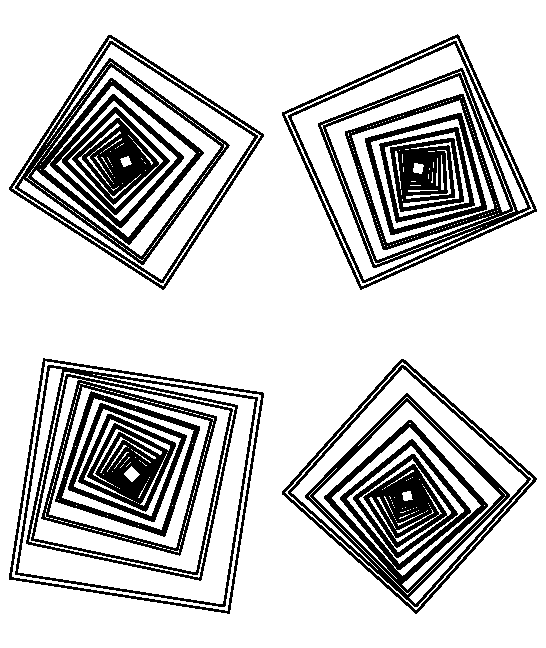
\includegraphics{figure/Rplot.pdf}

\end{frame}

\begin{frame}[fragile]{Beispieldaten bekommen}
\protect\hypertarget{beispieldaten-bekommen}{}

\begin{Shaded}
\begin{Highlighting}[]
\KeywordTok{library}\NormalTok{(osmdata)}
\end{Highlighting}
\end{Shaded}

\begin{verbatim}
## Data (c) OpenStreetMap contributors, ODbL 1.0. http://www.openstreetmap.org/copyright
\end{verbatim}

\begin{Shaded}
\begin{Highlighting}[]
\NormalTok{bb_poly <-}\StringTok{ }\KeywordTok{getbb}\NormalTok{(}\DataTypeTok{place_name =} \StringTok{"Amsterdam"}\NormalTok{, }
                 \DataTypeTok{format_out =} \StringTok{"polygon"}\NormalTok{)}
\end{Highlighting}
\end{Shaded}

\begin{Shaded}
\begin{Highlighting}[]
\NormalTok{ls <-}\StringTok{ }\KeywordTok{st_multilinestring}\NormalTok{(bb_poly)}
\end{Highlighting}
\end{Shaded}

\begin{Shaded}
\begin{Highlighting}[]
\NormalTok{pol <-}\StringTok{ }\NormalTok{sf}\OperatorTok{::}\KeywordTok{st_polygon}\NormalTok{(bb_poly)}
\KeywordTok{class}\NormalTok{(pol)}
\end{Highlighting}
\end{Shaded}

\begin{verbatim}
## [1] "XY"      "POLYGON" "sfg"
\end{verbatim}

\begin{Shaded}
\begin{Highlighting}[]
\NormalTok{bb_poly_ma <-}\StringTok{ }\KeywordTok{getbb}\NormalTok{(}\DataTypeTok{place_name =} \StringTok{"Mannheim"}\NormalTok{, }
                 \DataTypeTok{format_out =} \StringTok{"polygon"}\NormalTok{)}
\end{Highlighting}
\end{Shaded}

\end{frame}

\begin{frame}[fragile]{Das Ergebnis plotten}
\protect\hypertarget{das-ergebnis-plotten}{}

\begin{Shaded}
\begin{Highlighting}[]
\KeywordTok{plot}\NormalTok{(bb_poly_ma)}
\end{Highlighting}
\end{Shaded}

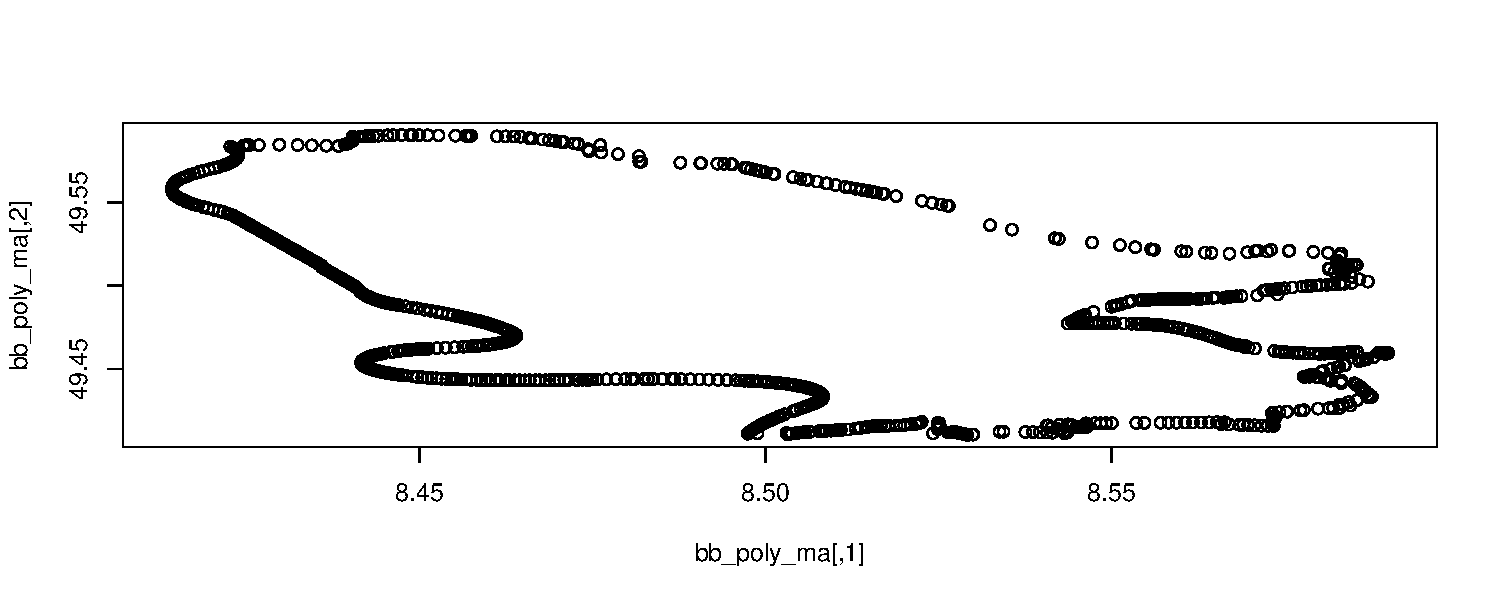
\includegraphics{simplefeatures_files/figure-beamer/unnamed-chunk-8-1.pdf}

\begin{Shaded}
\begin{Highlighting}[]
\CommentTok{# x <- osmdata_sf(pol)}
\end{Highlighting}
\end{Shaded}

\end{frame}

\begin{frame}[fragile]{Ein Beispieldatensatz}
\protect\hypertarget{ein-beispieldatensatz}{}

\begin{Shaded}
\begin{Highlighting}[]
\KeywordTok{demo}\NormalTok{(nc, }\DataTypeTok{ask =} \OtherTok{FALSE}\NormalTok{, }\DataTypeTok{echo =} \OtherTok{FALSE}\NormalTok{)}
\end{Highlighting}
\end{Shaded}

\begin{verbatim}
## Reading layer `nc.gpkg' from data source `D:\Eigene Dateien\Dokumente\R\win-library\3.5\sf\gpkg\nc.gpkg' using driver `GPKG'
## Simple feature collection with 100 features and 14 fields
## Attribute-geometry relationship: 0 constant, 8 aggregate, 6 identity
## geometry type:  MULTIPOLYGON
## dimension:      XY
## bbox:           xmin: -84.32385 ymin: 33.88199 xmax: -75.45698 ymax: 36.58965
## epsg (SRID):    4267
## proj4string:    +proj=longlat +datum=NAD27 +no_defs
\end{verbatim}

\end{frame}

\begin{frame}[fragile]{\href{https://r-spatial.github.io/sf/articles/sf5.html}{Graphiken
mit \texttt{sf}}}
\protect\hypertarget{graphiken-mit-sf}{}

\begin{Shaded}
\begin{Highlighting}[]
\KeywordTok{plot}\NormalTok{(nc)}
\end{Highlighting}
\end{Shaded}

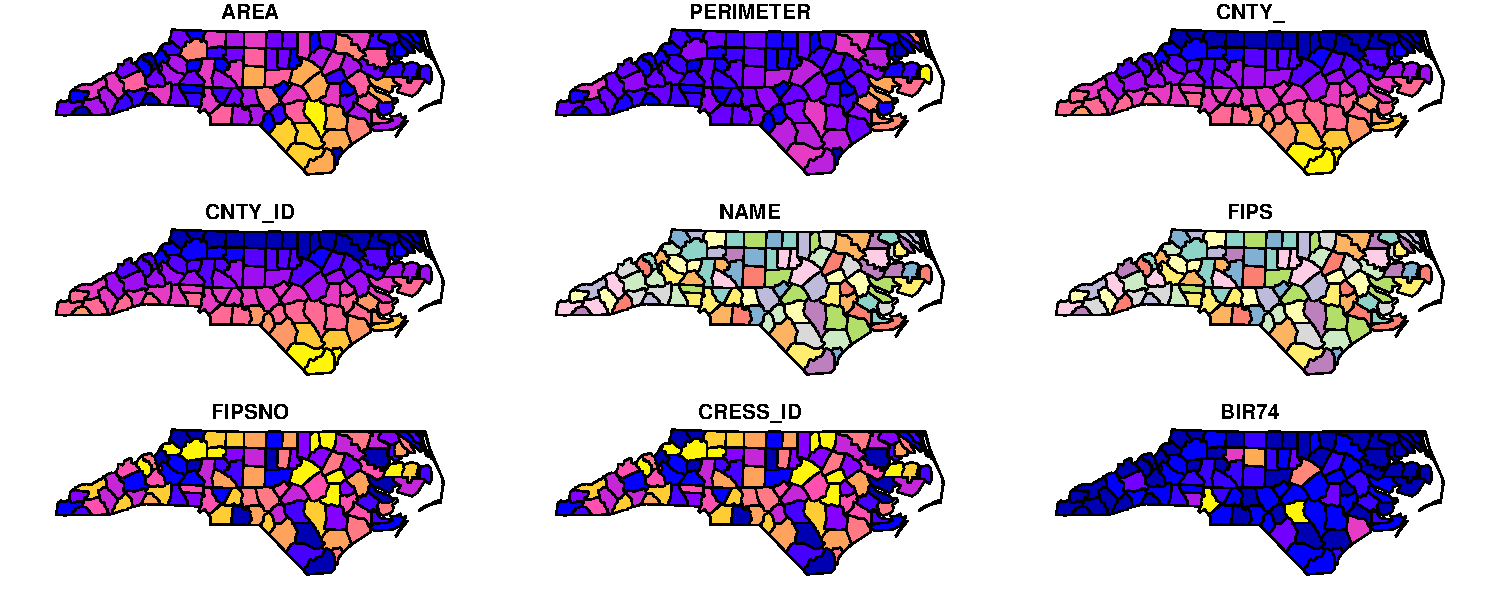
\includegraphics{simplefeatures_files/figure-beamer/unnamed-chunk-14-1.pdf}

\end{frame}

\begin{frame}[fragile]{\href{https://cran.r-project.org/web/packages/sf/vignettes/sf2.html}{Shapefiles
mit \texttt{sf} importieren}}
\protect\hypertarget{shapefiles-mit-sf-importieren}{}

\begin{Shaded}
\begin{Highlighting}[]
\NormalTok{lon <-}\StringTok{ }\KeywordTok{st_read}\NormalTok{(}\StringTok{"../data/london_sport.shp"}\NormalTok{)}
\end{Highlighting}
\end{Shaded}

\begin{verbatim}
## Reading layer `london_sport' from data source `D:\github\geocourse\data\london_sport.shp' using driver `ESRI Shapefile'
## Simple feature collection with 33 features and 4 fields
## geometry type:  POLYGON
## dimension:      XY
## bbox:           xmin: 503571.2 ymin: 155850.8 xmax: 561941.1 ymax: 200932.5
## epsg (SRID):    NA
## proj4string:    +proj=tmerc +lat_0=49 +lon_0=-2 +k=0.9996012717 +x_0=400000 +y_0=-100000 +ellps=airy +units=m +no_defs
\end{verbatim}

\end{frame}

\begin{frame}[fragile]{Das Shapefile plotten}
\protect\hypertarget{das-shapefile-plotten}{}

\begin{Shaded}
\begin{Highlighting}[]
\KeywordTok{plot}\NormalTok{(lon}\OperatorTok{$}\NormalTok{geometry)}
\end{Highlighting}
\end{Shaded}


\includegraphics{simplefeatures_files/figure-beamer/unnamed-chunk-18-1.pdf}

\end{frame}

\begin{frame}[fragile]{Daten vom Amsterdam Beispiel}
\protect\hypertarget{daten-vom-amsterdam-beispiel}{}

\begin{Shaded}
\begin{Highlighting}[]
\NormalTok{datm <-}\StringTok{ }\KeywordTok{st_read}\NormalTok{(}\StringTok{"../data/ams_centraal.osm"}\NormalTok{,}\StringTok{"multipolygons"}\NormalTok{)}
\end{Highlighting}
\end{Shaded}

\begin{verbatim}
## Reading layer `multipolygons' from data source `D:\github\geocourse\data\ams_centraal.osm' using driver `OSM'
## Simple feature collection with 2796 features and 25 fields
## geometry type:  MULTIPOLYGON
## dimension:      XY
## bbox:           xmin: 4.874776 ymin: 52.36088 xmax: 4.929755 ymax: 52.39393
## epsg (SRID):    4326
## proj4string:    +proj=longlat +datum=WGS84 +no_defs
\end{verbatim}

\end{frame}

\begin{frame}[fragile]{\href{https://cran.r-project.org/web/packages/sf/vignettes/sf3.html}{Die
Funktion \texttt{st\_geometry}}}
\protect\hypertarget{die-funktion-st_geometry}{}

\begin{Shaded}
\begin{Highlighting}[]
\NormalTok{geom_datm <-}\StringTok{ }\KeywordTok{st_geometry}\NormalTok{(datm)}
\KeywordTok{plot}\NormalTok{(geom_datm)}
\end{Highlighting}
\end{Shaded}


\includegraphics{simplefeatures_files/figure-beamer/unnamed-chunk-20-1.pdf}

\end{frame}

\begin{frame}[fragile]{Die Häuser auswählen}
\protect\hypertarget{die-hauser-auswahlen}{}

\begin{Shaded}
\begin{Highlighting}[]
\KeywordTok{library}\NormalTok{(dplyr)}
\NormalTok{buis <-}\StringTok{ }\NormalTok{datm }\OperatorTok\StringTok{ }\KeywordTok{select}\NormalTok{(building)}
\KeywordTok{plot}\NormalTok{(buis)}
\end{Highlighting}
\end{Shaded}

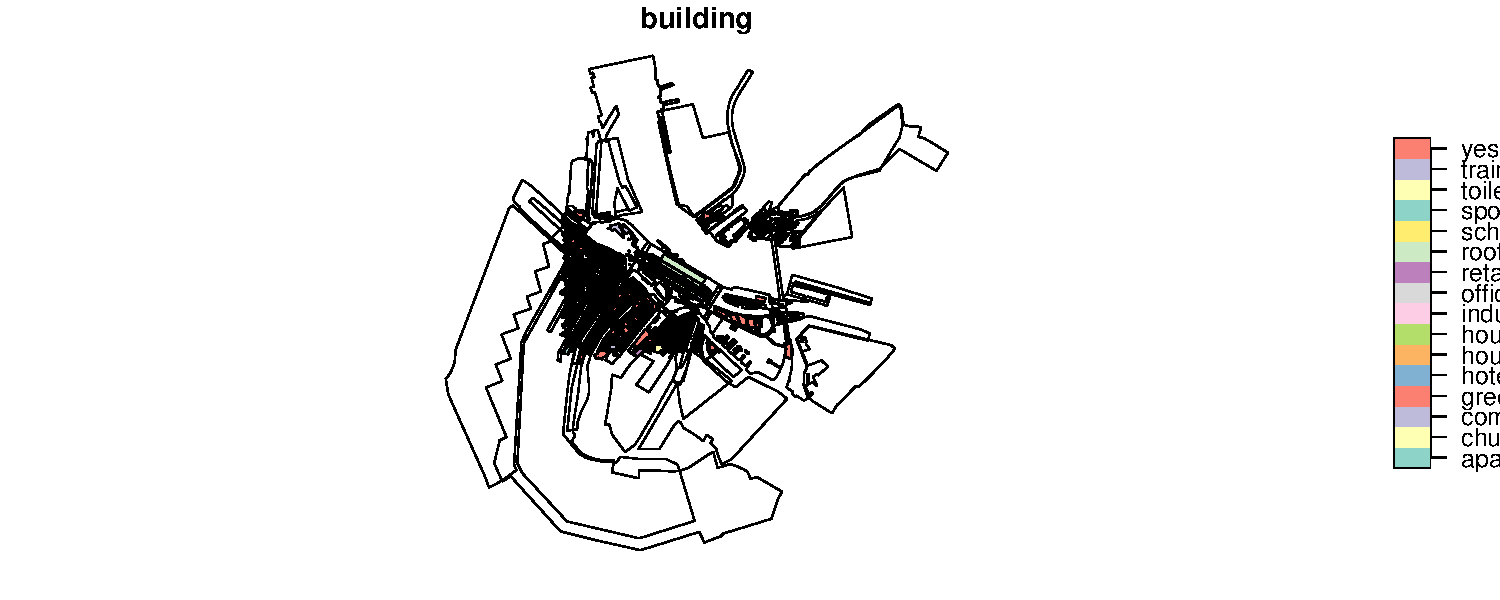
\includegraphics{simplefeatures_files/figure-beamer/unnamed-chunk-21-1.pdf}

\end{frame}

\begin{frame}[fragile]{Welche Häusertypen gibt es?}
\protect\hypertarget{welche-hausertypen-gibt-es}{}

\begin{Shaded}
\begin{Highlighting}[]
\NormalTok{buis2 <-}\StringTok{ }\NormalTok{datm }\OperatorTok\StringTok{ }\NormalTok{as.data.frame }\OperatorTok\StringTok{ }\KeywordTok{select}\NormalTok{(building)}
\end{Highlighting}
\end{Shaded}

\begin{Shaded}
\begin{Highlighting}[]
\NormalTok{datbuis <-}\StringTok{ }\NormalTok{datm[, }\StringTok{"building"}\NormalTok{, drop =}\StringTok{ }\OtherTok{TRUE}\NormalTok{]}
\KeywordTok{plot}\NormalTok{(datbuis)}
\end{Highlighting}
\end{Shaded}

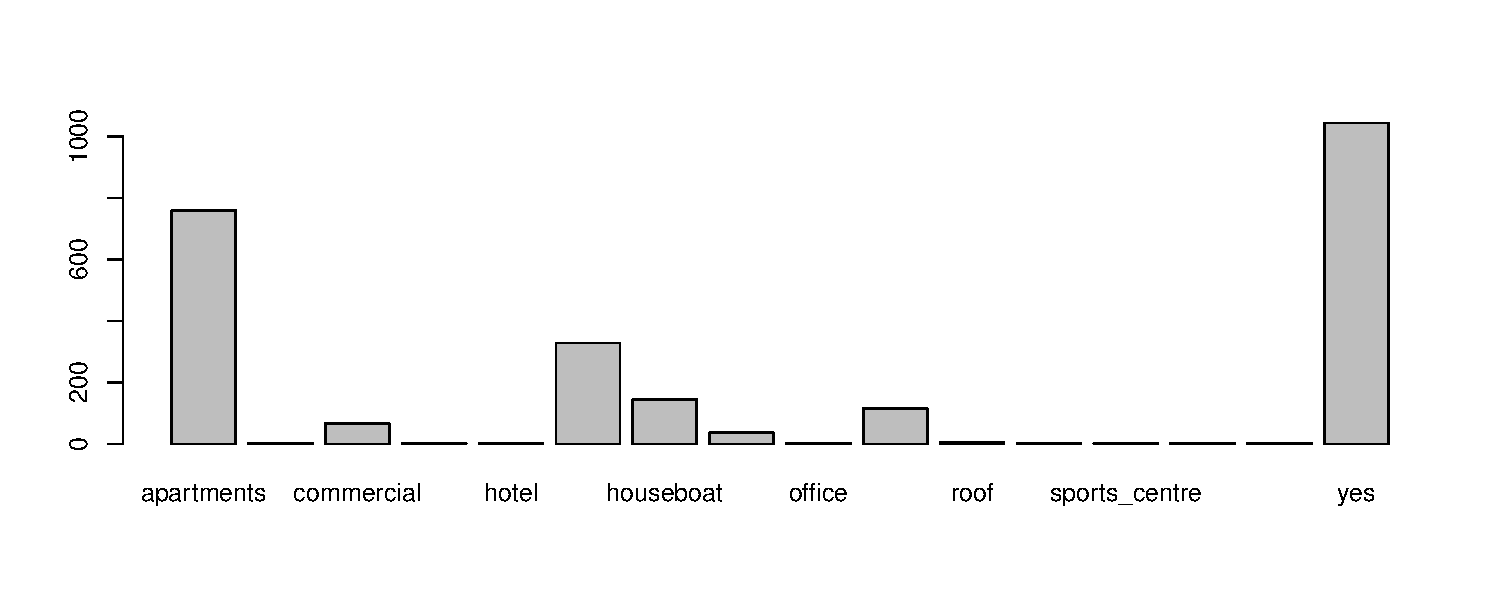
\includegraphics{simplefeatures_files/figure-beamer/unnamed-chunk-23-1.pdf}

\end{frame}

\begin{frame}[fragile]{}
\protect\hypertarget{section}{}

\begin{Shaded}
\begin{Highlighting}[]
\NormalTok{houses <-}\StringTok{ }\NormalTok{datm[datm}\OperatorTok{$}\NormalTok{building }\OperatorTok{==}\StringTok{ "house"}\NormalTok{,]}
\KeywordTok{class}\NormalTok{(houses)}
\end{Highlighting}
\end{Shaded}

\begin{verbatim}
## [1] "sf"         "data.frame"
\end{verbatim}

\begin{Shaded}
\begin{Highlighting}[]
\NormalTok{## [1] "sf"         "data.frame"}
\NormalTok{dhous <-}\StringTok{ }\NormalTok{datm[houses,]}
\end{Highlighting}
\end{Shaded}

\begin{verbatim}
## although coordinates are longitude/latitude, st_intersects assumes that they are planar
\end{verbatim}

\begin{Shaded}
\begin{Highlighting}[]
\KeywordTok{plot}\NormalTok{(dhous}\OperatorTok{$}\NormalTok{geometry)}
\end{Highlighting}
\end{Shaded}


\includegraphics{simplefeatures_files/figure-beamer/unnamed-chunk-24-1.pdf}

\begin{Shaded}
\begin{Highlighting}[]
\KeywordTok{plot}\NormalTok{(}\KeywordTok{st_geometry}\NormalTok{(houses))}
\end{Highlighting}
\end{Shaded}


\includegraphics{simplefeatures_files/figure-beamer/unnamed-chunk-25-1.pdf}

\end{frame}

\begin{frame}[fragile]{\href{https://cran.r-project.org/web/packages/sf/vignettes/sf4.html}{Alle
Häuser herausnehmen}}
\protect\hypertarget{alle-hauser-herausnehmen}{}

\begin{Shaded}
\begin{Highlighting}[]
\NormalTok{houses <-}\StringTok{ }\NormalTok{datm[datm}\OperatorTok{$}\NormalTok{building }\OperatorTok\StringTok{ }\KeywordTok{c}\NormalTok{(}\StringTok{"house"}\NormalTok{,}\StringTok{"yes"}\NormalTok{,}
                                    \StringTok{"apartments"}\NormalTok{),]}
\KeywordTok{plot}\NormalTok{(}\KeywordTok{st_geometry}\NormalTok{(houses))}
\end{Highlighting}
\end{Shaded}


\includegraphics{simplefeatures_files/figure-beamer/unnamed-chunk-26-1.pdf}

\end{frame}

\begin{frame}{Die Vignetten für das Paket \texttt{sf}}
\protect\hypertarget{die-vignetten-fur-das-paket-sf}{}

\url{https://r-spatial.github.io/sf/reference/st_as_sf.html}

\url{https://r-spatial.github.io/sf/reference/st_read.html}

\url{https://r-spatial.github.io/sf/articles/sf1.html}

\end{frame}

\end{document}
